\documentclass[10pt, margin=1mm]{standalone}

\usepackage{amsmath}
\usepackage{tikz}
\usetikzlibrary{calc, tikzmark, shapes, shapes.arrows, arrows, 3d, positioning}

\begin{document}
\begin{tikzpicture}[arrow/.style={black, thick,->,>=latex}, remember picture]
	\tikzset{xshift=.5cm}
	\Large
	\node (psi) at (4.75,0) {
		$\psi($%
			\subnode{psi_x}{$\boldsymbol{\mathrm{x}}$}, 
			\subnode{psi_omega}{$\boldsymbol{\mathrm{\Omega}}$}, 
			\subnode{psi_nu}{$\nu$}, 
			\subnode{psi_t}{$t$})
	}; 
	\tiny
	\node[anchor=north, label=south:3D hydro grid] (space) at ($(psi) + (-3cm,-1.25cm)$) {
		\begin{tikzpicture}[scale=.175]
			\foreach \x in{0,...,4}
			{   
				\draw (0,\x ,4) -- (4,\x ,4);
				\draw (\x ,0,4) -- (\x ,4,4);
				\draw (4,\x ,4) -- (4,\x ,0);
				\draw (\x ,4,4) -- (\x ,4,0);
				\draw (4,0,\x ) -- (4,4,\x );
				\draw (0,4,\x ) -- (4,4,\x );
			}
		\end{tikzpicture}
	}; 
	\draw[arrow] (psi_x) to (space); 
	\node[anchor=north, label=south:2D angular grid] (angular) at ($(psi) + (-1cm,-1.5cm)$) {
		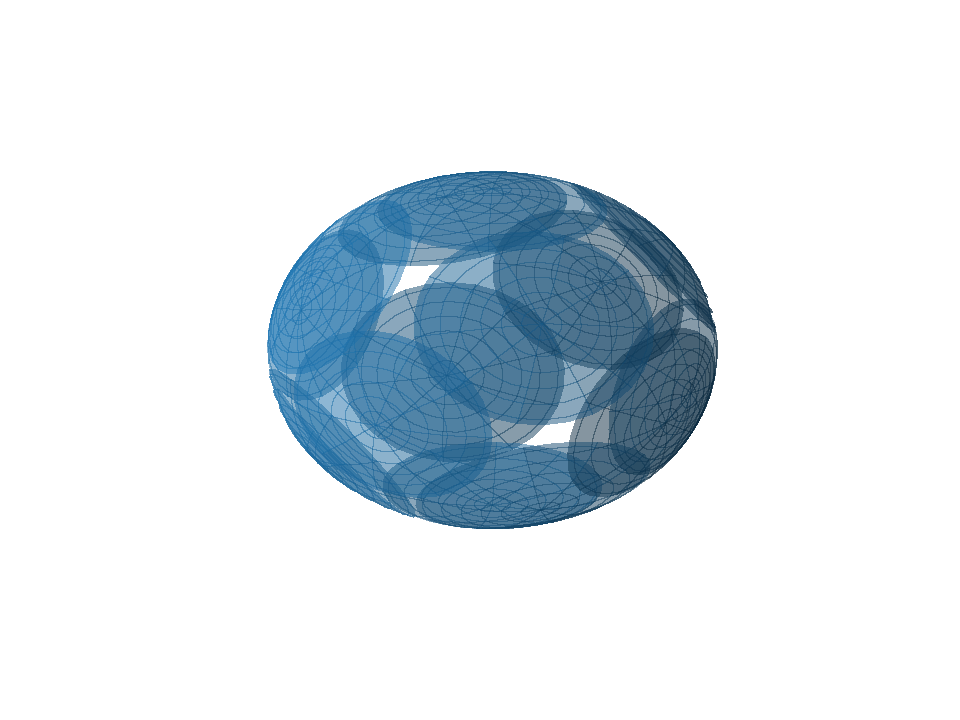
\includegraphics[width=2.8cm, trim=0 75 0 75, clip]{../data/img/sphere.pdf}
	};
	\draw[arrow] (psi_omega) to (angular); 
	\node[anchor=north, label=south:1D frequency grid] at ($(psi)+(1.25cm,-1.75cm)$) (energy) {
		\begin{tikzpicture}[scale=.15]
			\draw[step=1] (0,-.2) grid (10,.2); 
		\end{tikzpicture}
	};
	\draw[arrow] (psi_nu) to ([yshift=1.5em]energy); 
	\node[single arrow, draw, minimum height=6em, single arrow head extend=1ex,inner sep=1ex, fill=black, shape border rotate=90, label=south:1D time dependence] at ($(psi)+(3.25cm,-.75cm)$) (time) {}; 
	\draw[arrow] (psi_t) to ([xshift=-1em,yshift=-1.5em]time); 
\end{tikzpicture}

\end{document}